\documentclass[conference]{IEEEtran}
\IEEEoverridecommandlockouts
% The preceding line is only needed to identify funding in the first footnote. If that is unneeded, please comment it out.
\usepackage{cite}
\usepackage{amsmath,amssymb,amsfonts}
\usepackage{algorithmic}
\usepackage{graphicx}
\usepackage{textcomp}
\usepackage{xcolor}
\usepackage{subfig}
\usepackage{booktabs}
\def\BibTeX{{\rm B\kern-.05em{\sc i\kern-.025em b}\kern-.08em
    T\kern-.1667em\lower.7ex\hbox{E}\kern-.125emX}}
\begin{document}

\title{Detect the Decoy Routing System Based on Routing and Timing Attacks\\
%{\footnotesize \textsuperscript{*}Note: Sub-titles are not captured in Xplore and
%should not be used}
%\thanks{Identify applicable funding agency here. If none, delete this.}
%}
%\author{\IEEEauthorblockN{1\textsuperscript{st} Given Name Surname}
%\IEEEauthorblockA{\textit{dept. name of organization (of Aff.)} \\
%\textit{name of organization (of Aff.)}\\
%City, Country \\
%email address}
%\and
%\IEEEauthorblockN{2\textsuperscript{nd} Given Name Surname}
%\IEEEauthorblockA{\textit{dept. name of organization (of Aff.)} \\
%\textit{name of organization (of Aff.)}\\
%City, Country \\
%email address}
%\and
%\IEEEauthorblockN{3\textsuperscript{rd} Given Name Surname}
%\IEEEauthorblockA{\textit{dept. name of organization (of Aff.)} \\
%\textit{name of organization (of Aff.)}\\
%City, Country \\
%email address}
%\and
%\IEEEauthorblockN{4\textsuperscript{th} Given Name Surname}
%\IEEEauthorblockA{\textit{dept. name of organization (of Aff.)} \\
%\textit{name of organization (of Aff.)}\\
%City, Country \\
%email address}
%\and
%\IEEEauthorblockN{5\textsuperscript{th} Given Name Surname}
%\IEEEauthorblockA{\textit{dept. name of organization (of Aff.)} \\
%\textit{name of organization (of Aff.)}\\
%City, Country \\
%email address}
%\and
%\IEEEauthorblockN{6\textsuperscript{th} Given Name Surname}
%\IEEEauthorblockA{\textit{dept. name of organization (of Aff.)} \\
%\textit{name of organization (of Aff.)}\\
%City, Country \\
%email address}
}
\maketitle

\begin{abstract}
Decoy Routing is a novel approach for circumventing the Internet censorship. It uses the end-to-middle proxy technology to embed the censored data into the traffic of overt sites covertly, and achieves the goal of censorship circumvention without being detected by the censor. Some research works have been proposed to confirm the effectiveness of decoy routing. But these works have not fine-grained covered the following situations:1)possible abnormal browsing behaviors when the decoy router could not supply the decoy client with enough covert data;2)overhead  to keep consistent with the overt flow when retransmission occurs;3) the extraordinarily long duration of decoy routing session because of merging multiple web access in one single session. 4)possible differences in the bit stream between initial and retransmitted packets when a retransmisstion occurs.In summary, to prompt the decoy routing systems safer and perfect, in this paper we propose detection methods from the above four perspectives. By simulation, we demonstrate that an active censor can detect the decoy routing session by catching the abnormal browsing behaviors caused by his active attacks or due to some other situations when the decoy router could not provide enough covert data. In addition, we show that an active censor could force the retransmittion of decoy session and challenge the consistency of bit stream between the initial and retransmitted packets. What's more, we also find that there is a large difference on end-to-end latency of retransmitted packets between decoy routing flow and overt flow, which could provide basis for the censor to detect the decoy routing flow. Finally, we demonstrate the exraordinarily long duration of decoy routing session could be a remarkable feature which may be a criterion for the censor the launch further attacks.
\end{abstract}

\begin{IEEEkeywords}
Decoy Routing, BGP, Censorship, Slitheen
\end{IEEEkeywords}

\section{Introduction}
Nowadays, there has been an upward trend of repressive regimes(hereafter called the warden) which implement the internet censorship to hinder people from sharing idea, information and speech online freely\cite{b1}\cite{b2}\cite{b3}. The main techniques of internet censorship include IP address blacklist, DNS hijacking, deep-packet inspection and so on\cite{b4}\cite{b5}. It is with no doubt that the internet censorship is a common threat to all the users, since it may damage data integrity and confidentiality and infringe individual privacy. To help network user to bypass the network censorship and protect their information security, several kinds of censorship circumvention tools have been designed, such as VPNs, Tor, and Psiphon\cite{tor}\cite{vpn1}\cite{vpn2}\cite{b9}. However, these tools require the user to connect to the proxy server first, which is vulnerable to IP block attack. And the IP block attack is one of the most common and basic means, which is widely available on the Internet. Thus a novel method called decoy routing systems is proposed. Instead of connecting to the proxy server based on IP address directly, the decoy routing systems just require the user to establish some TLS sessions whose routing path contains the decoy router, which is called end-to-middle(E2M) proxying. As described in figure 1, the decoy routing system or E2M proxying  is composed of three components: the decoy routing client, the decoy routing router(hereafter called decoy routers) and the external overt sites(web sites that are not banned from access, and the path between the client and them contains some decoy routers). In order to access blocked sites decoy users generate tagged traffic to overt sites to which the network paths contain some deployed decoy routers. If the tag is recognied by the decoy router, the decoy router will learn the wish to access blocked data of the current user. Then the decoy router will keep on observing the subsequent handshake messages to collect enough secret to intercept the current session successfully. Once the decoy router finishes intercepting the session, it will remind the decoy user of its existence and open a proxy connection to the censored sites. Compared to traditional circumvention means, decoy routing deploys the circumvention device on the middle of the network paths than on the end host or servers. As a result, the users need not to connect the decoy router directly based on IP address, but just establish connection crossing the decoy router. The decoy traffic will signal the decoy router to take man-in-the-middle actions, proxying the connection to its real destination. By this 
technology, the decoy routing is able to resistant IP address block, which is common means in the internet censorship. Decoy routing was first proposed by \cite{cirripede}, \cite{curveball}, \cite{telex} in 2011. Initially there were three main problems for the first generation of decoy routing systems:in-line flow block(i.e., the decoy router tears down the oringinal overt connection and personates the overt site by forging corresponding packets with reasonable TCP state), latency vulnerability(i.e., the latency of intercepted session is different from the that of the regular overt session) and path symmetry(i.e., the upstream and downstream traffic should both traverse the same decoy router). In RAD\cite{rad}, Schuchard et al. demonstrated that by simply analyze the end-to-end lantency the censor could not only detect the decoy routing traffic, but also determine the website that the client was accessing. To conter this kind of timing attack, a state-of-the-art method called Slitheen was proposed. Unlike tradditional decoy routing systems, in Slitheen the decoy router does not block the overt flow directly. Alternatively the decoy router keeps the overt session running as normal and store the censored data of the covert sites in some queues. When one packet of the overt session passess through it, the decoy router will fetch the stored data from the queue and replace the overt downstream packet with the fetched data properly. In this way Slitheen avoids the waiting delay to receive the censored data from the covert site and thus keep the latency of the covert traffic almost the same as the overt traffic. Since the packet is really generated by the overt site, the TCP state and the other flow fingerprint will be the same as regular overt traffic. Thus Slitheen also resistants to the attacks based on challenging the consistency of the tcp state of current session, which enables the Slitheen to imitate the original overt session perfectly. However, Slitheen still have some drawbacks which may cause the user detected by the censor and even bring the users high risk. To develop safeguard decoy routing techniques for censorship circumvention issues, we propose some detection methods toward Slitheen in this paper.
\begin{figure}[htbp]
	\centerline{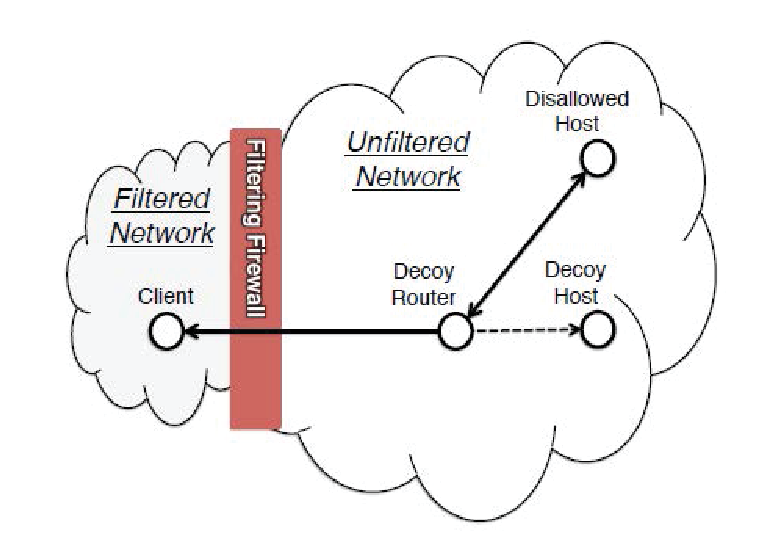
\includegraphics[width=7cm]{Figure1.eps}}
	\caption{Architecture of decoy routing system.}
	\label{fig}
\end{figure} 
The essence of the Slitheen is that using multiple overt sessions to carry the censored data of covert session back. To provide enough packets for the decoy router to replace, the browsing behavior of the Slitheen users may be quite different from regular users. For instance, in Slitheen the client continued to establish sessions toward one specific overt sites time and time again, which is remarkable feature.  To the best of our knowledge, the abnormal browsing behavior of Slitheen has not been well researched. In this paper, we first propose a detection method toward Slitheen from the aspect of the browsing behavior. The abnormal browsing behaviors may be caused by active attacks launched by the censor, or the network congestion between the decoy router and the covert site. Since Slitheen does not solve the challenge of path symmetry(i.e., it can just work when the upstream and downstream traffic both traverse the decoy router), an active censor could launch routing attack to force Slitheen users produce some abnormal browsing behaviors. In RAD\cite{rad}, Schuchard et al. proposed a routing attacks that force the upstream traffic to bypass the decoy router to achieve the goal of preventting the users from contacting with the decoy routing system. This attack is also effective for Slitheen, since Slitheen needs the upstream traffic to recognize the tag and learn the covert request. As a result, the Slitheen user may establish connections to some overt sites frequently, which is remarkable to the censor. Meanwhile, the influnces of manipulating the downstream traffic to Slitheen has not been studied. If the downstream traffic does not pass through the decoy router, it will have no chance to inject the stored censored data back, which may cause some abnormal reactions from the user. Although some previous decoy routing systems such as Tapdance\cite{tapdance} and Rebound\cite{rebound} can work normally when the downstream traffic does not cross the decoy router, these two works cound not imitate the overt traffic as well as Slitheen. Tapdance leaves the connection between the client and the overt site open, which is vulnerable to replay attacks. Rebound requires the user to send equal amount of upstream data to the downstream data they want to receive, which is contradictory with the fact that the ratio between upstream traffic and downstream traffic is very low in web browsing scenes. Finally, if there is a network congestion between the covert site and the decoy router, the decoy user can not receive complete data to open the target web page within some reasonable time, which may also cause some abnormal behaviors. To make Slitheen more perfect and safe, we evaluate the perfomance of Slitheen under the condition that the downstream route path get changed and the network congestion respectively in this paper. We show that all the above situation may cause abnormal browsing behaviors  of Slitheen user, which enables the censor to detect the usage of Slitheen.
On the other hand, packet loss is very common in the network. When some packets of a session get lost, the TCP protocol will retransmit the lost packets to the client. By default, the retransmitted packets should be the same as the droped ones. Thus an active censor could drop some suspicious packets in order to force the retransmission of these packets and compare the retransmitted packets with the dropped ones. If the retransmitted packets are not the same as the dropped ones, the censor will determine that current flow is using some censorship circumvention technology. As a result, in Slitheen the decoy router should save all the replaced packets in order to handle such kind of drop attacks. Since Slitheen is designed to respond to national level opponents, the number of replaced packets could be pretty large at certain time. Thus when retransmission occurs, the time overhead of looking up the right replaced packets should not be ignored. As far as we know, the retransmission overhead of decoy routing has not been covered. We analyze the influnces of this overhead and take it as another detection metric in this paper.
Once again, the decoy usersusually utilize the one established decoy session to access multiple censored web sites in practical applications. Thus the total duration of the decoy session may be much longer than normal ones. At the same time, a state-level adversary has the ability to collect enough data to estimate the accessing duration distribution to given overt site of users within its jurisdiction. So if the duration of some session is far beyond normal range, the warden will certainly suspect that the user is using some censorship circumvention tools, which causes then censor to launch some further attacks to determine whether current session is Slitheen session. As far as we know, none of the previous decoy routing system has covered this problem. Then thirdly, we will demonstrate the feasibility of this attack towards Slitheen in this paper. 

% Slitheen does not solve the challenge of path symmetry(i.e., it can just work when the upstream and downstream traffic both traverse the decoy router). In RAD\cite{rad}, Schuchard et al. proposed a routing attacks that force the upstream traffic to bypass the decoy router to achieve the goal of preventting the users from contacting with the decoy routing system. This attack is also effective for Slitheen, since Slitheen needs the upstream traffic to recognize the tag and learn the covert request. However, the influnces of manipulating the downstream traffic has not been studied. If the downstream traffic does not pass through the decoy router, it will have no chance to inject the stored censored data back, which may cause some abnormal reactions from the user. Although some previous decoy routing systems such as Tapdance\cite{tapdance} and Rebound\cite{rebound} can work normally when the downstream traffic does not cross the decoy router, these two works cound not imitate the overt traffic as well as Slitheen. Tapdance leaves the connection between the client and the overt site open, which is vulnerable to replay attacks. Rebound requires the user to send equal amount of upstream data to the downstream data they want to receive, which is contradictory with the fact that the ratio between upstream traffic and downstream traffic is very low in web browsing scenes. To make Slitheen more perfect and safe, we evaluate the perfomance of Slitheen under the condition that the downstream route path get changed in this paper.
%most of current decoy routing systems can only work under the condition of path symmetry and thus are vulnerable to some routing attacks. Since the decoy routing does not explicitly require users to connect the decoy router using IP addresses, a routing capable adversary may leverage the routing attacks to bypass the decoy router and then block the decoy routing system. For instance, in RAD\cite{rad}, the censor manipulates the upstream BGP routes so that any traffic origins from its jurisdiction does not transit through any decoy ASes(Autonomous system deploying decoy routers). As a result, the internal users are prevented from contacting the decoy routing system. To counter the routing attacks such as RAd, many means have been proposed. For example, Nasr et al designed a downstream-only decoy routing mechanism that just requires downstream decoy routing traffic transit through decoy router to resistant to RAD in waterfall\cite{warterfall}; Wustrow et al. proposed
%TapDance\cite{tapdance}, which just requires the upstream decoy routing flow transit the decoy router. In Tapdance, the user kept the overt %site silent by sending TCP ACK packets whose ACK numbers are higher than overt site’s TCP SND.NXT. And during the silence time of overt site, %the decoy router sends back the requested page by generating some spoofed responses from the overt site; Daniel Ellard et al designs a new decoy system called Rebound, which can work under the path asymmetric condition in \cite{rebound}.Rebound embedded the covert data in the upstream traffic which will cause the overt site generate an error message. The over site will attach the embedded covert data in the error message automatically, so Rebound is resistant to attacks of manipulating downstream packet route. Except Rebound, all the other works above are decoy routing systems that resistant manipulating upstream traffic attack, and the effect of manipulating the downstream traffic has not been fully researched. \cite{cirripede}, \cite{curveball}, \cite{tapdance}, \cite{telex}and \cite{slitheen} assumed that the downstream decoy routing traffic must cross the decoy ASes, and \cite{warterfall} assumed that the warden could not manipulate downstream traffic per-source (e.g.,the censoring ISP has to re-route either all or none of its downstream traffic through each of its Internet provider ASes), which is too coarse-grained. Even in Rebound, the decoy routing is very fragile, since the rebound decoy router will be blacklisted by the overt site for continuous sending error causing HTTP get requests, which is similar as HTTP flooding attack. If route path of the downstream traffic changes and does not cross the decoy router any more, the path-changing will stop the user from receiving remaining decoy packets needed to open the web page successfully. Then the user must try to make new opportunities to enable the downstream traffic transit through the decoy router again. We call this decoy routing path-changing abnormal behavior. From the point of the warden, he can actively move the downstream traffic to other clean paths(paths do not cross any decoy ASes), and catch the association of the decoy routing path-changing abnormal behavior and his manipulation. In this paper we will first give a detection method according to the decoy routing path-changing abnormal behaviors . Apart from this, RAD also indicates that the end-to-end delay of decoyed session is quite different from overt session, which may expose the decoy users. To mend this timing drawback, Slitheen was designed\cite{slitheen}, which used the caching and replacement mechanism to perfectly imitate the overt traffic on the aspect of end-to-end delay and tcp session state. However, if packet loss occurs, the overt site should retransmit lost packets according to the tcp protocol. And If the retransmitted packet is different from the former replaced one, the warden will doubt that the user may be using decoy routing systems. To make things worse, the warden can actively force the overt site to retransmit packets by dropping some suspicious packets and simply compare the former and retransmitted packets bit by bit to judge if the two packets are the same. To overcome this attack, the decoy router in Slitheen should save all the packets which it has modified before for possible retransmission before corresponding session is released. Because the decoy routing is designed to defend against sate-level adversary, the amount of replaced packets will be very huge at certain moment. Thus the lookup overhead of finding the right replaced packets should not be neglected, which may cause clear difference on end-to-end delay between normal and Slitheen sessions. So secondly, we propose another decoy routing detection method based on the delay difference of retransmission packets. Once again, the decoy usersusually utilize the one established decoy session to access multiple forbidden web sites in practical applications. Thus the total duration of the decoy session may be much longer than normal ones. At the same time, a state-level adversary has the ability to collect enough data to estimate approximate accessing duration distribution from its jurisdiction to given overt site. So if the duration of some session is far beyond normal range, the warden will certainly suspect that the user is using some censorship circumvention tools. As far as we know, none of the previous decoy routing system has covered this problem. Then thirdly, we will demonstrate the feasibility of this attack in this paper. 

In summary, to make the decoy routing more robust and much safer, we point out the vulnerability of existing decoy routing system by giving detection methods from the following three perspectives:
\begin{itemize}
\item The abnormal user behaviors caused by path-change of the downstream decoy sessions or network congestion between the decoy router and the censored site. There hasn’t been any fine-grain research in this field. It is possible for a state-level adversary to leverage BGP poisoning attack to change both the upstream and downstream path of specific session. The network congestion is common in the Internet at certain time. The abnormal behaviors of decoy users caused by these factors have not been fully researched.
\item The delay difference of retransmission. Although Slitheen has achieved the goal of perfect imitation of the end-to-end delay between decoy sessions and overt sessions, the overhead caused by the replacement mechanism has not been taken into consideration. It is obvious that the session state and replaced packets should be saved for possible retransmission. The huge amount of replaced packets must produce a lookup overhead that should not be ignored.
\item The abnormally long accessing duration of decoy routing systems. If the user accesses multiple covert sites using one decoy connection, the total duration will be much longer than that of just accessing single web site. Previous research has not covered this problem, and we will verify the possibility of detecting decoy routing systems using this property.
\end{itemize}

The rest of this paper is organized as follows: In section 2, we introduce some research works related to our work. In section 3, we give the problem statement and threat model. In section 4, we analysis probable abnormal results caused by routing attacks. In section 5, we verify the feasibility of timing attacks including delay difference of retransmission and comparison of accessing duration between normal and decoy routing sessions. In section 6, we conclude our paper.


\section{Related Work}

\subsection{Traditonal Censorship Circumvention Tools}
Traditional censorship circumvention tools mainly depend on the simple proxy technology. These systems set up proxy servers outside the censor's domain. Users establish encrypted connection with the proxy server and use the encrypted connection to hide their real destination. VPNs\cite{vpn1}\cite{vpn2} are just this kind of circumvention tools. On the other hand, Tor\cite{tor}is a more robust system which providing stronger anonymity by expanding single relay proxy to three ones. In Tor, the proxy servers are thousands of volunteer users(i.e., the Tor user can be the Tor proxy server at the same time ) so that the Tor user could choose muiltiple proxy servers to relay their traffic to some censored sites. In both situation, the warden could find the user has established a encrypted connection to the relay proxy, and learn the IP address of the proxy(in Tor the censor could learn the IP address of the first proxy which is called entry relays ). So the warden could defeat these systems by simply blacklisting the IP address the relay proxies.

Domain fronting\cite{domainfonting} is another technique that circumvents Internet censorship. This technique works by setting different domain names at different layers of communication. An innocuous domain name is used to initialize the connection, which can be seen by the censor from the DNS request and the TLS Server Name Indication in clear-text form. After the establishment of the encrypted HTTPS connection, the real censored domain name is sent in the HTTP Host header in ciphertext form, which is invisible to censors. Then the innocuous websites proxy the censored data back to the user. In this way Domain fronting is able to resist IP block attacks. The key point of Domain fronting is that it uses some popular and influential websites(such as google.com and Amazon, etc.) as its proxy server and blocking these websites will cause demages that cannot be ignored to the censor. But the CPU and bandwidth cost charged by the websites hosting Domain fronting service is very high, which hinders it from being widely deployed.

CDNBrowsing\cite{CDNbrowsing}\cite{cdnbrowsing} is a similar censorship circumvention approach. It works based on the fact that some censored sites can be accessed from the the public content-delivery networks(CDN networks) directly(such as Akamai). And again blocking this kind of public content-delivery sites will cause loss to the censor so that the censor is unwilling to block the sites completely. However, using CDNbrowsing the users could only access the limited censored sites that host themselves on the CDN networks.

%The IEEEtran class file is used to format your paper and style the text. All margins, 
%column widths, line spaces, and text fonts are prescribed; please do not 
%alter them. You may note peculiarities. For example, the head margin
%measures proportionately more than is customary. This measurement 
%and others are deliberate, using specifications that anticipate your paper 
%as one part of the entire proceedings, and not as an independent document. 
%Please do not revise any of the current designations.
\subsection{Decoy Routing Systems}
To defend against the IP blocking attack, decoy routing system was first proposed in 2011\cite{cirripede}\cite{telex}\cite{curveball}. The first generation decoy routing systems require the decoy router to block the flow in-line and the symmetry of network paths, which is vulnerable to many attacks. For instance, in RAD\cite{rad}, Schuchard et al. blocked and detected the decoy routing systems by two main methods: routing attack and timing attack. On the aspect of routing attack, Schuchard et al. assumed a routing capable adversary that could manipulate the BGP routes between the censored area and the overt sites. The censor actively chose some clean paths(paths that does not contain any decoy routers) to transmit the upstream traffic, which blocked the decoy routing system by preventing decoy users from contacting with decoy routers.  The essence of routing attack is to destroy the symmetry of the network path. To deploy decoy routing systems under path asymmetry situation, some follow-up research works were carried out. Tapdance\cite{tapdance}and Rebound\cite{rebound} are two main decoy routing systems that only need the upstream traffic to cross the decoy router, while the Waterfall\cite{warterfall} is the decoy routing system that can work normally when only the downstream traffic traverse the decoy router. In Tapdance, the user keep the overt site silent by sending TCP ACK packets whose ACK numbers are higher than overt site’s TCP SND.NXT. And during the silence time of overt site, the decoy router sends back the censored page by generating some spoofed response packets that seems to be sent by the overt site. Tapdance, however, can not resist to the RAD attack, since the decoy router needs to check the existence of tag embedded in the upstream traffic. Meanwhile the sequence number of spoofed packet is also different from the tcp state of the real overt site, and the warden could actively replay a TCP ACK packet with a stale sequence number to find this discrepancy. As discussed above, Rebound may cause doubt from both the warden and overt sites. It generates HTTP get error time and time again to fetch the complete censored data back, which is similar to the HTTP flooding attack. And the ratio between upstream and downstream traffic is much higher than normal web browsing traffic. This abnormal phenomenon will certainly cause doubt of the censor. Waterfall\cite{warterfall} defeats the RAD attack by deploying the decoy router only on the downstream path. It applied the same covert chanel as Rebound to carry the tag and the covert access requests to the decoy router through the rebounded downstream traffic. Waterfall, however, can not resist to the dowstream routing attack. It was assumed in Waterfall that the warden could only manipulate downstream path by applying per-source rules, which are too coarse-grained. The influnces of the downstream path change of an ongoing session was not covered in Waterfall. Another work called Gossip\cite{gossip} designed a gossip protocol to add asymmetry to previously symmetric decoy routing systems. Once again, Gossip did not take the manipulation of downstream path into consideration.

On the aspect of timing attack, RAD indicated that first generation decoy routing systems were also vulnerable to timing attacks. The end-to-end latency of covert and overt communications was very different. To perfectly imitate time pattern of the overt session, Slitheen maintained the intercepted overt connection, and used the storing and replacement methods to provide proxy service. In Slitheen, the decoy router stores covert data in several queues. When the downstream packet of overt session transit through it, the decoy router fetches the corresponding covert data from the queues and replaces the overt packet with the fetched covert data. By doing so, Slitheen enables the decoy router to avoid waiting for the arriving of the covert data. Thus in Slitheen, the latency difference between two corresponding overt and covert sessions is just the processing delay of each packet, which is not large enough to differentiate two sessions. What’s more, Slitheen avoids tearing down the overt tcp connection, which enable it to resist to tcp replay attack. But Slitheen did not cover the adversary who is able to manipulate downstream routing path and the latency overhead produced by looking up the proper saved packets, which may be a definite characteristic for the censor to detect it. Finally, Houmansadr et al argued that it would impose tremendous costs if the warden launched RAD attacks in \cite{truecost}; Nasr et al.\cite{game} performed a game theoretic analysis to optimize the deployment of decoy routers with the existence of the decoy adversary while Previous deployment research was under the non-adversary condition\cite{optimize}\cite{combinatoric}.
\subsection{BGP Routing}
The Internet is composed of many ASes(Autonomous systems). An AS is a set of routers and IP addressess which are under unified management. The routing decision between ASes is made by the Boader Gateway Protocol(BGP). Thus BGP is the actually routing protocol between different ASes. Through BGP different ASes exchange information about route to certain ASes and learn the routing path to different destinations. In particular, each BGP router may receive multiple paths  with different properties between two ASes on Internet, and it can make their own policy to choose the “best” path they believe. These policies gradually extend from simply choosing the “fastest” or “shortest” routes to making routing decision based on the complicated relationships between ASes. There are three economic relationships between ASes: provider, peer, customer. If A pays B to carry traffic, then A is a customer of B, and B is a provider of A. If two ASes make a agreement to carry the traffic of each other freely, then they are peer of each other(A and B stands for different ASes here). These economic relatioships are main factors considered by the ASes: A customer will not advertise routes to its providers except those it or its customers originate. A provider will advertise all routes to all ASes to any of its (paying) customers. An AS never redistributes routes from one of its providers to another. These are basic policies what is known as “valley-free routing” \cite{valley}. Generally speaking, the route decision strategy should comply with the “valley-free” principle. So the routing relationships among Ases are predictable, and people could infer the path along which the traffic will be transmitted to a specific network destination. Qiu and Gao\cite{path1} and Mao, Qiu, Wang, and Zhang\cite{path2} give designs about inferring the path between two endpoints on the Internet without requiring access to each other. From the point of censor, BGP routing is similar to source-routing , i.e., the routing path consists of several relay ASes, and the censor knows every relay node(ASes) of each given path. As described in RAD, the censor could use path-pruning method to confirm which AS has deployed the decoy router(hereafter called decoy AS), and launch RAD attacks by choosing clean BGP route paths to transmit data. Besides "valle-free routing", the common decision fators for choosing the best path are illustrated in table I. From table I we can learn that BGP is vulnerable to BGP poisoning attacks, in which an attacker could induce the BGP router to choose his expected path by forging routing information according to the routing decision priority. So it is possible for state-level censor to manipulate the routing path in BGP routing.
\begin{table}[htbp]
	\caption{BGP decision factors for path choosing}
	\centering
	\begin{tabular}{l}		
	\toprule
	1 Ignore if next hop unreachable\\
	2 Prefer locally originated networks\\
	3 Business preference (highest Local-Pref)\\
	4 Shortest AS path\\
	5 Prefer lowest Origin\\
	6 Prefer lowest MED\\
	7 Prefer eBGP over iBGP\\
	8 Prefer nearest next hop\\
	9 Prefer lowest Router-ID or Originator-ID\\
	10 Prefer shortest Cluster-ID-List\\
	11 Prefer lowest neighbor address\\
	%	Works & Sampling & Purpose & Theory\\
	%	\midrule
	%	Our Work & Part of RSU & Recover Trajectory & Matrix Completion\\
	%	Yan et al. 2012 & RSU & Minimize the Number of RSU & Greedy Algorithm \\
	%	Tomer et al. 2007 & Video & Microscopic Traffic Behavior & Locally Weighted Regression \\
	%	Xin et al. 2008 & Video & Unsafe Driver Behavior & Bi-level Optimization  \\
	\bottomrule
	\end{tabular}

\end{table}
\subsection{User Browsing Behavior Analysis}


\section{Problem Statement and Threat Model}
In this paper, we focus on the following problem: a user uses decoy routing mechanism to circumvent the censorship of the censor. He aims to access some web sites without being detected by the censor of his host network. Meanwhile, the censor wants to distinguish the traffic of decoy-routing from the normal ones. Since the decoy routing is designed to defend against the adversary of nation-state level power, we assume that the warden controls the internet infrastructure within his jurisdiction. He has the privilege of monitoring, blocking, modifying, replaying and injecting traffic within this region. We also assume that the censor can not control the end equipment within his jurisdiction, and all the end terminals run under the direction of their own users. On the other hand, we assume that the censor has limited rights outside his jurisdiction, which means that the warder can not control any infrastructure and sites that may be used in the decoy routing systems. At the same time, the censor will not block all the traffic since the internet connectivity can bring him economic and social benefits. So we assume the warden uses the blacklist rather than whitelist mechanism to filter the traffic, which means that the warden just blocks the traffic which is against the filtering rules. As mentioned in RAD attack, we assume that the warden has the ability to launch routing attack, which may change the upstream or downstream path of the traffic originating from his jurisdiction, and the warden is aware of the set of ASes deploying decoy routers and the location of the decoy routers. Finally, we assume that the warden allows users to communicate using the encrypted communication protocols such as TLS/SSL for the purpose of protecting personal privacy, but he can selectively manipulate the connection or shut the communication down.
\section{Catch the Abnormal Browsing Behaviors}
In this section we propose our detection methods by catching abnormal browsing behavior caused by routing attacks or network congestion.
\subsection{Forcing Path to Change}
As described in RAD and Waterfall, it is possible for the censor to change the downstream routes in order to bypass certain decoy routers. One of the most well-known methods is BGP hijack attack. BGP hijacking (sometimes referred to as prefix hijacking, route hijacking or IP hijacking) is the illegitimate takeover of groups of IP addresses by corrupting Internet routing tables maintained using the Border Gateway Protocol (BGP). In BGP hijacking, the censor could forge and advertise more shorter or more specific BGP routes to victim AS, and then hijack the traffic passing through the victim AS(can be decoy AS). Besides BGP hijacking, the censor can leverage the loop prevent mechanism of BGP to avoid downstream traffic traversing decoy ASes. For instance, a censor could achieve the goal in Waterfall like this: let AS$_{C}$ be the ASes that the censor control or possess, and AS$_{D}$ be the ASes deploying decoy router. So the censor can make the downstream traffic bypass the AS$_{D}$ by advertising the specific-designed BGP route AS$_{C}$-AS$_{D}$-AS${_{C}}$ to every neighbor of AS$_{D}$. If the neighbors of AS$_{D}$ enables the loop prevent mechanism, it will not advertise any route of AS$_{C}$ to AS$_{D}$. Then the AS$_{D}$ will not know any route to AS$_{C}$, so any downstream traffic to AS$_{C}$ will not transit through AS$_{D}$. In summary, there are indeed some methods for the censor to force the routing path to change when the route is decided by BGP.
\subsection{Catch the Path-changing Abnormal Browsing Behaviors }
As discussed in RAD, if the censor has already known the location of the decoy router, and he has multiple BGP paths to certain destination, then he can launch some active routing attacks to prevent the upstream or downstream traffic from passing through the decoy ASes. In Slitheen, covert data was sent back in the downstream traffic of decoy sessions. If the downstream traffic does not cross the decoy router, covert data will be blocked. In detail, the censor could actively change the routing path of the  downstream traffic when the decoy session is going on. From then on, the decoy user can not use the path-changed decoy connection to receive the remaining covert data. Thus he has to establish a new intercepted connection with the overt site (e.g. refresh the web page )or take any other actions which could make opportunities for the overt site to transmit downstream data along the path containing the decoy ASes again. No matter in which way, the frequency of the packet sending will increase dramatically. On the other hand, the change of downstream path will not affect the normal user, since the required data of normal user can also be received through other clean paths. We call this phenomenon decoy routing path-changing abnormal behavior. More importantly, there is an obvious association between the abnormal behavior of the decoy user and the routing attacks of the censor: the increase of packet sending frequency follows the routing attack closely. We believe that this association may become a criterion to detect the decoy router users. 

In order to verify the feasibility of this attack, we have performed the following simulations illustrated in figure 2. We use the NS2 simulation platform to make the simulations as following: Firstly we deployed one node (node User) to stand for the network users which may not only run normal network applications but also run Siltheen. Secondly we deployed two nodes to stand for overt site(node Overt) and covert site(node Covert) respectively. Then we deployed some relay nodes working as relay nodes. These relay nodes include one special node(node Relay Station) to work as decoy router and the remaining nodes to work as normal relay nodes. And we established one clean path and one decoy path(path contains decoy relay station) respectively. The detail simulation parameters are described in table II. We let the user node run Ftp traffic and Slitheen traffic to get the same amount of packets back from the overt and covert node simultaneously. To achieve the effect of manipulating paths, we selectively turned down and turned on corresponding links: first, the link between User and R\_2 will be cut down.So all the traffic will be forwarded along the decoy path. Then at 10 s the link between User and R\_1 will be cut down and the link between User and R\_2 will be turn on. As a result, the Slitheen traffic will not cross the decoy router any more, and the abnormal behavior may take place. At 25s the link between User and R\_1 will be turn on  and the link between User and R\_2 will be cut down. Thus the Slitheen traffic will transit through the decoy router again. And the simulation lasts for 100 seconds. We take packet-sending frequency as the main metric. As shown in figure 3, after the decoy path was shut down the difference on packet-sending frequency between Ftp and Slitheen traffic became significant, since the Slitheen user is not able to receive the remaining packets, and tries to establish new decoy connection towards overt site. 


\begin{figure}[htbp]
	\centerline{\includegraphics[width=7cm]{Figure2.eps}}
	\caption{Topology of manipulating routing paths simulations.}
	\label{fig}
\end{figure}

\begin{figure}[htbp]
	\centerline{\includegraphics[width=7cm]{Figure3.eps}}
	\caption{Abnormal behaviors of manipulating downstream path.}
	\label{fig}
\end{figure}
\subsection{Catch Network Congestion Abnormal Behaviors}
In some situations the decoy router can not supply the decoy user with enough covert data. For instance, there is a congestion between the decoy router and the covert site, or the destination covert site is too busy to response current request. If the client could not receive total packets to open the censor site within normal browsing duration, the decoy users will probably try to establish another decoy connection or reflesh current web page to open the censored page again. No matter in which way, they will increase the packet-sending frequency to implement their plan. But normal users will not take these actions and thus a differentiation is caused, which can be used by the censor as a detection metric. Although it is not likely for the censor to cause the network congestion between any censored site and decoy router, he can choose some important sites and increase the session response time by attacks such as DDos attack actively. Then the censor could detect the user accessing the victim sites by observing the difference on the packet-sending frenquency or some other abnormal behaviors. 

We also make a simulation to evaluate the inffluences of such attack by setting fail replacing rate of decoy router to the behaviors of Slitheen user. We achieve this by setting the fail replacing rate of decoy router. In detail, we recorded the results of fail rate from 20\% to 40\%, figure 4 shows the results. it is obvious that the packet-sending frequency is also much larger than normal users, if there is not enough data for the decoy router to replace with. So we believe that the censor can successfully detect the use of decoy routing if he launches some attacks to enlarge the latency between the covert site and the decoy router.

 \begin{figure}[htbp]
 	\centering
 	\subfloat[]{
 		\label{fig.sub.1}
 		\includegraphics[width=5cm]{Figure4a.eps}}
 	\subfloat[]{
 		\label{fig.sub.2}
 		\includegraphics[width=5cm]{Figure4b.eps}}
 	%\subfloat[]{
 	%	\label{fig.sub.3}
 	%	\includegraphics[width=5cm]{Figure4c.eps}}
 	\caption{CDF of retransmission end-to-end delay of normal and Slitheen users}
 	\label{fig.lable}
 \end{figure}

\section{Timing Attacks}
\subsection{Session Duration Attacks}
Typically, the decoy users may use the single decoy connection to access multiple censored sites, which is quite different from normal web page browsing process. The most obvious difference of the decoy session is the session duration. Using decoy routing, the duration is the sum of each sub browsing duration, so the duration of decoy routing session is usually significant longer than that of normal browsing sessions. But all of the previous decoy routing works did not cover this problem. Considering that the decoy routing is designed to defend state-level adversary, so the state-level censor is able to collect enough data to estimate the reasonable range of browsing duration of specific website, and he can set threshold according to the estimated duration range. As a result, although Slitheen could imitate the overt session perfectly, it can not eliminate the fact that the session duration is far more than the normal duration range of the other users, which may cause the censor launch other attacks to verify whether the decoy routing is working. To counter this attack, the decoy user may establish multiple decoy sessions and use each decoy session to access single censored sites like normal users. The censor, however, can add up the number of established decoy sessions and the total duration of each decoy session within general web page browsing time(e.g., 30 minutes). In the most extreme cases the censor could take every session traversing decoy AS as a decoy session, and accumulate the duration together. Let D$_{di}$ be the ith decoy session duration found within the predefined web page browsing time, N be the number of established sessions that traverses the decoy AS, then the total duration of decoy sessions can be expressed as $\sum_{n=1}^ND_{di}$. This value will be compared to the duration threshold. If it is much larger than the threshold, the corresponding user will be suspected, and the censor will launch other active attacks to further certificate it. To verify the feasibility of such attacks, we have made a test like followings:we use Slitheen to access multiple web sites randomly, and recorded the duration of Slitheen session. Then we directly accessed the corresponding sites and recorded the separate session duration. Then we calculated the max duration of the normal session, and set the threshold as four times of the max duration. Then we compared the duration of Slitheen session to the threshold. This test was repeated 100 times. The results were shown in figure 5. We can obviouly find that there is large difference between the two session durations.

\begin{figure}[htbp]
	\centerline{\includegraphics[width=7cm]{Figure4.eps}}
	\caption{CDF of session duration between Slitheen and normal sessions.}
	\label{fig}
\end{figure}
\subsection{Retransmission Attacks}
In Slitheen, covert data is sent back by replacing the overt site packets. In order to resistant the forced retransmission attack, the decoy router should save every changed packet before the corresponding session is tore down. So the decoy router should open up a space to save all the modified packets of the current decoy routing sessions. It is obvious that the amount of these packets is very huge, since the decoy routing is designed to provide nation level service. When a modified packet needs to be retransmitted, the decoy router should find the right packet among all the saved modified packets. Suppose there are M tagged flows running at specific moment, and each tagged flow contains N${_{i}}$ modified packets, the time overhead of lookup will be ${M+N{_{i}}}$ in the worst case, which should not be neglected bacause the M and ${N_{i}}$ are both very large. Meanwhile, the retransmission packets of normal user will not follow this process, thus there will be a significant difference on the end-to-end delay between the normal and decoy routing users. So the censor can selectively drop some packets and compare the end-to-end delay of the retransmission packets. If the delay changed obviously, then it is likely that the corresponding user is using decoy routing. What's more, the censor is able to increase the total amount of the decoy session actively, which will enlarge the delay difference of the retransmission packets between the normal and decoy users. For instance, the censor could utilize the end terminals to establish huge amount of decoy session handled by a specific decoy router; and the censor could prevent the decoy router from releasing specific session using long connection mechanism of TCP. We have performed simulations to evaluate the difference of end-to-end delay of retransmission packets in decoy routing and non-decoy sessions. As illustrated in figure 6, we first deployed one node to work as internet user(node User), several nodes to work as ordinary routers(R\_1, R\_2...R\_n), one specific node to work as decoy router(node RelayStation), and two nodes to work as overt(node Overt) and covert sites(node Covert). We added traffic from Ftp\_1 to Ftp\_m gradually to put the stress on the network. The first  traffic will start at the beginning and the rest will start three seconds later, respectively. The router R\_1 to R\_n is simulating the different covert and overt websites. With the different n, the packet will travel different distances in the network, which enable us to measure the influences under diffrent end-to-end session delays. Figure 7 gives the simulation results. We find the lookup overhead is sufficient to distinguish Slitheen traffic.

\begin{figure}[htbp]
	\centerline{\includegraphics[width=7cm]{Figure5.eps}}
	\caption{Simulation deployment for retransmission.}
	\label{fig}
\end{figure}

\begin{figure}[htbp]
	\centering
	\subfloat[]{
		\label{fig.sub.1}
		\includegraphics[width=5cm]{Figure6a.eps}}
	\subfloat[]{
		\label{fig.sub.2}
		\includegraphics[width=5cm]{Figure6b.eps}}
	%\subfloat[]{
	%	\label{fig.sub.3}
	%	\includegraphics[width=5cm]{Figure6c.eps}}
	\caption{CDF of retransmission end-to-end delay of normal and Slitheen users}
	\label{fig.lable}
\end{figure}
\section{Bit Comparison Attacks}
Slitheen is state-of-the-art decoy routing system, which has strong resistance to flow fingerprint analysis. It uses replacement mechanism instead of directly in-line blocking the overt traffic, which can imitate the overt traffic perfectly. However, the replacement based mechanism is also fragile when the censor is able to change the downstream path. Although data transmitted by Slitheen has been encrypted, the censor can still compare the bit of packets directly in the mac layer to verify if two packets have the same bit stream. Generally speaking, the initial packet and the retransmitted packet of the same session with the same sequence number should have the same packet data, thus the bit stream should be the same, too. since the retransmission is realized automatically by the TCP, which just fetches previously cached packets from its buffer and sends them again. So we can follow the steps below to verify if the packets have been replaced, and further verify if the user is using Slitheen:
\begin{enumerate}
	\item The censor saves one or more packets of the suspect session.
	\item The censor drops the TCP ACK pakcets of these saved suspect packets to force the retransmission of these packets.
	\item The censor moves the downstream path to other clean path.
	\item After receiving the retransmitted packets, the censor compares the retransmitted packet to the previously saved one of the same sequence number bit by bit. If all the bits are the same, then the packet is not replaced. Otherwise, the packet may be replaced by Slitheen.
\end{enumerate}
In summary, TLS protocol could only prevent the censor from knowing the content of the packets. It could not prevent the censor from verifying the  consistency between any packet. So the censor could detect the Slitheen session by forcing the overt site to retransmit some packets, and challenging the consistency of the initial and retransmitted packets.
%Before you begthe ASes deploying decoy router. So the warden can make the downstream traffic bypass thein to format your paper, first write and save the content as a 
%separate text file. Complete all content and organizational editing before 
%formatting. Please note sections \ref{AA}--\ref{SCM} below for more information on 
%proofreading, spelling and grammar.

%Keep your text and graphic files separate until after the text has been 
%formatted and styled. Do not number text heads---{\LaTeX} will do that 
%for you.

%\subsection{Abbreviations and Acronyms}\label{AA}
%Define abbreviations and acronyms the first time they are used in the text, 
%even after they have been defined in the abstract. Abbreviations such as 
%IEEE, SI, MKS, CGS, ac, dc, and rms do not have to be defined. Do not use 
%abbreviations in the title or heads unless they are unavoidable.

%\subsection{Units}
%\begin{itemize}
%\item Use either SI (MKS) or CGS as primary units. (SI units are encouraged.) English units may be used as secondary units (in parentheses). An exception would be the use of English units as identifiers in trade, such as ``3.5-inch disk drive''.
%\item Avoid combining SI and CGS units, such as current in amperes and magnetic field in oersteds. This often leads to confusion because equations do not balance dimensionally. If you must use mixed units, clearly state the units for each quantity that you use in an equation.
%\item Do not mix complete spellings and abbreviations of units: ``Wb/m\textsuperscript{2}'' or ``webers per square meter'', not ``webers/m\textsuperscript{2}''. Spell out units when they appear in text: ``. . . a few henries'', not ``. . . a few H''.
%\item Use a zero before decimal points: ``0.25'', not ``.25''. Use ``cm\textsuperscript{3}'', not ``cc''.)
%\end{itemize}

%\subsection{Equations}
%Number equations consecutively. To make your 
%equations more compact, you may use the solidus (~/~), the exp function, or 
%appropriate exponents. Italicize Roman symbols for quantities and variables, 
%but not Greek symbols. Use a long dash rather than a hyphen for a minus 
%sign. Punctuate equations with commas or periods when they are part of a 
%sentence, as in:
%\begin{equation}
%a+b=\gamma\label{eq}
%\end{equation}

%Be sure that the 
%symbols in your equation have been defined before or immediately following 
%the equation. Use ``\eqref{eq}'', not ``Eq.~\eqref{eq}'' or ``equation \eqref{eq}'', except at 
%the beginning of a sentence: ``Equation \eqref{eq} is . . .''

%\subsection{\LaTeX-Specific Advice}

%Please use ``soft'' (e.g., \verb|\eqref{Eq}|) cross references instead
%of ``hard'' references (e.g., \verb|(1)|). That will make it possible
%to combine sections, add equations, or change the order of figures or
%citations without having to go through the file line by line.

%Please don't use the \verb|{eqnarray}| equation environment. Use
%\verb|{align}| or \verb|{IEEEeqnarray}| instead. The \verb|{eqnarray}|
%environment leaves unsightly spaces around relation symbols.

%Please note that the \verb|{subequations}| environment in {\LaTeX}
%will increment the main equation counter even when there are no
%equation numbers displayed. If you forget that, you might write an
%article in which the equation numbers skip from (17) to (20), causing
%the copy editors to wonder if you've discovered a new method of
%counting.

%{\BibTeX} does not work by magic. It doesn't get the bibliographic
%data from thin air but from .bib files. If you use {\BibTeX} to produce a
%bibliography you must send the .bib files. 

%{\LaTeX} can't read your mind. If you assign the same label to a
%subsubsection and a table, you might find that Table I has been cross
%referenced as Table IV-B3. 

%{\LaTeX} does not have precognitive abilities. If you put a
%\verb|\label| command before the command that updates the counter it's
%supposed to be using, the label will pick up the last counter to be
%cross referenced instead. In particular, a \verb|\label| command
%should not go before the caption of a figure or a table.

%Do not use \verb|\nonumber| inside the \verb|{array}| environment. It
%will not stop equation numbers inside \verb|{array}| (there won't be
%any anyway) and it might stop a wanted equation number in the
%surrounding equation.

%\subsection{Some Common Mistakes}\label{SCM}
%\begin{itemize}
%\item The word ``data'' is plural, not singular.
%\item The subscript for the permeability of vacuum $\mu_{0}$, and other common scientific constants, is zero with subscript formatting, not a lowercase letter ``o''.
%\item In American English, commas, semicolons, periods, question and exclamation marks are located within quotation marks only when a complete thought or name is cited, such as a title or full quotation. When quotation marks are used, instead of a bold or italic typeface, to highlight a word or phrase, punctuation should appear outside of the quotation marks. A parenthetical phrase or statement at the end of a sentence is punctuated outside of the closing parenthesis (like this). (A parenthetical sentence is punctuated within the parentheses.)
%\item A graph within a graph is an ``inset'', not an ``insert''. The word alternatively is preferred to the word ``alternately'' (unless you really mean something that alternates).
%\item Do not use the word ``essentially'' to mean ``approximately'' or ``effectively''.
%\item In your paper title, if the words ``that uses'' can accurately replace the word ``using'', capitalize the ``u''; if not, keep using lower-cased.
%\item Be aware of the different meanings of the homophones ``affect'' and ``effect'', ``complement'' and ``compliment'', ``discreet'' and ``discrete'', ``principal'' and ``principle''.
%\item Do not confuse ``imply'' and ``infer''.
%\item The prefix ``non'' is not a word; it should be joined to the word it modifies, usually without a hyphen.
%\item There is no period after the ``et'' in the Latin abbreviation ``et al.''.
%\item The abbreviation ``i.e.'' means ``that is'', and the abbreviation ``e.g.'' means ``for example''.
%\end{itemize}
%An excellent style manual for science writers is \cite{b7}.

%\subsection{Authors and Affiliations}
%\textbf{The class file is designed for, but not limited to, six authors.} A 
%minimum of one author is required for all conference articles. Author names 
%should be listed starting from left to right and then moving down to the 
%next line. This is the author sequence that will be used in future citations 
%and by indexing services. Names should not be listed in columns nor group by 
%affiliation. Please keep your affiliations as succinct as possible (for 
%example, do not differentiate among departments of the same organization).

%\subsection{Identify the Headings}
%Headings, or heads, are organizational devices that guide the reader through 
%your paper. There are two types: component heads and text heads.

%Component heads identify the different components of your paper and are not 
%topically subordinate to each other. Examples include Acknowledgments and 
%References and, for these, the correct style to use is ``Heading 5''. Use 
%``figure caption'' for your Figure captions, and ``table head'' for your 
%table title. Run-in heads, such as ``Abstract'', will require you to apply a 
%style (in this case, italic) in addition to the style provided by the drop 
%down menu to differentiate the head from the text.

%Text heads organize the topics on a relational, hierarchical basis. For 
%example, the paper title is the primary text head because all subsequent 
%material relates and elaborates on this one topic. If there are two or more 
%sub-topics, the next level head (uppercase Roman numerals) should be used 
%and, conversely, if there are not at least two sub-topics, then no subheads 
%should be introduced.

%\subsection{Figures and Tables}
%\paragraph{Positioning Figures and Tables} Place figures and tables at the top and 
%bottom of columns. Avoid placing them in the middle of columns. Large 
%figures and tables may span across both columns. Figure captions should be 
%below the figures; table heads should appear above the tables. Insert 
%figures and tables after they are cited in the text. Use the abbreviation 
%``Fig.~\ref{fig}'', even at the beginning of a sentence.

%\begin{table}[htbp]
%\caption{Table Type Styles}
%\begin{center}
%\begin{tabular}{|c|c|c|c|}
%\hline
%\textbf{Table}&\multicolumn{3}{|c|}{\textbf{Table Column Head}} \\
%\cline{2-4} 
%\textbf{Head} & \textbf{\textit{Table column subhead}}& \textbf{\textit{Subhead}}& \textbf{\textit{Subhead}} \\
%\hline
%copy& More table copy$^{\mathrm{a}}$& &  \\
%\hline
%\multicolumn{4}{l}{$^{\mathrm{a}}$Sample of a Table footnote.}
%\end{tabular}
%\label{tab1}
%\end{center}
%\end{table}

%\begin{figure}[htbp]
%\centerline{\includegraphics{fig1.png}}
%\caption{Example of a figure caption.}
%\label{fig}
%\end{figure}

%Figure Labels: Use 8 point Times New Roman for Figure labels. Use words 
%rather than symbols or abbreviations when writing Figure axis labels to 
%avoid confusing the reader. As an example, write the quantity 
%``Magnetization'', or ``Magnetization, M'', not just ``M''. If including 
%units in the label, present them within parentheses. Do not label axes only 
%with units. In the example, write ``Magnetization (A/m)'' or ``Magnetization 
%\{A[m(1)]\}'', not just ``A/m''. Do not label axes with a ratio of 
%quantities and units. For example, write ``Temperature (K)'', not 
%``Temperature/K''.

%\section*{Acknowledgment}

%The preferred spelling of the word ``acknowledgment'' in America is without 
%an ``e'' after the ``g''. Avoid the stilted expression ``one of us (R. B. 
%G.) thanks $\ldots$''. Instead, try ``R. B. G. thanks$\ldots$''. Put sponsor 
%acknowledgments in the unnumbered footnote on the first page.
\section{Conclusion}
In this paper, we have introduced a threat model that the censor can manipulate the route path of both upstream and downstream decoy traffic. Based on this model, we have proposed and verified decoy routing detection methods from three perspective. Firstly, we have taken fine-grained research on the influences of the downstream path change and analyzed the decoy routing path-changing abnormal behavior. We have found that the censor could leverage active routing attacks to force the browsing behaviors of decoy users to be completely different from normal ones; Secondly, we have analyzed the security from the timing property of decoy routing sessions. We have evaluated that the lookup overhead of retransmission packets do affect the end-to-end delay significantly. And the duration of decoy routing session is much larger than normal sessions, which could become a criterion for the censor to launch further attacks. Thirdly, we have designed a novel detection method by comparing original and retransmitted packets bit by bit, which will give a conclusive evidence of using decoy routing system;  Simulations have been implemented and the results demonstrate effectiveness of our detection method. In summary, we believe that these works will help the decoy routing systems become more robust and safer, which will provide safe and efficient proxy service for censored people.
%\section*{References}

%Please number citations consecutively within brackets \cite{b1}. The 
%sentence punctuation follows the bracket \cite{b2}. Refer simply to the reference 
%number, as in \cite{b3}---do not use ``Ref. \cite{b3}'' or ``reference \cite{b3}'' except at 
%the beginning of a sentence: ``Reference \cite{b3} was the first $\ldots$''

%Number footnotes separately in superscripts. Place the actual footnote at 
%the bottom of the column in which it was cited. Do not put footnotes in the 
%abstract or reference list. Use letters for table footnotes.

%Unless there are six authors or more give all authors' names; do not use 
%``et al.''. Papers that have not been published, even if they have been 
%submitted for publication, should be cited as ``unpublished'' \cite{b4}. Papers 
%that have been accepted for publication should be cited as ``in press'' \cite{b5}. 
%Capitalize only the first word in a paper title, except for proper nouns and 
%element symbols.

%For papers published in translation journals, please give the English 
%citation first, followed by the original foreign-language citation \cite{b6}.

\begin{thebibliography}{00}
\bibitem{b1} China blocks VPN services that let Internet users get around censorship.\\ http://www.scmp.com/news/china/article/1689961/china-blocks-vpn-services-let-internet-users-$\backslash$around-censorship. Online Article.
\bibitem{b2} Colin Lecher. How Iran Censors The Internet.\\ http://www.popsci.com/technology/article/2013-03/how-iran-censors-internet-infographic. Online Article.
%\bibitem{b3} Colin Lecher. Internet censorship reaching dangerous levels in Turkey.\\ http://www.todayszaman.com/national${_}$internet-censorship-reaching-dangerous-levels-in-turkey${_}$393727.html. Online Article
\bibitem{b3} Phil Sands. Syria Tightens Control over Internet.\\ http://www.thenational.ae/news/world/middle-east/syria-tightens-control-over-internet. Online Article.
\bibitem{b4} Christopher S. Leberknight, Mung Chiang, and Felix Ming Fai Wong. 2012. A\\
Taxonomy of Censors and Anti-Censors Part II: Anti-Censorship Technologies.\\
Int. J. E-Polit. 3, 4 (Oct. 2012), 20–35. https://doi.org/10.4018/jep.2012100102
\bibitem{b5}Michael Carl Tschantz, Sadia Afroz, Vern Paxson, et al. 2016. SoK: Towards\\
Grounding Censorship Circumvention in Empiricism. In IEEE S\&P. 914–933
\bibitem{tor} Roger Dingledine, Nick Mathewson, and Paul Syverson. 2004. Tor: The Secondgeneration\\
Onion Router. In USENIX Security.
\bibitem{vpn1} Daiyuu Nobori and Yasushi Shinjo. 2014. VPN Gate: A Volunteer-Organized\\
Public VPN Relay System with Blocking Resistance for Bypassing Government\\
Censorship Firewalls.. In NSDI. 229–241
\bibitem{vpn2} Vasile C Perta, Marco V Barbera, Gareth Tyson, Hamed Haddadi, and Alessandro\\
Mei. 2015. A glance through the VPN looking glass: IPv6 leakage and DNS\\
hijacking in commercial VPN clients. PoPETs 2015, 1 (2015), 77–91.
\bibitem{b9} Jeffrey Jia and Patrick Smith. Psiphon: Analysis and Estimation. http://www.cdf.\\
toronto.edu/~csc494h/reports/2004-fall/psiphon-ae.html.
\bibitem{rad} Schuchard M, Geddes J, Thompson C, et al. Routing around decoys[C]//Proceedings of the 2012 ACM conference on Computer and\\ communications security. ACM, 2012: 85-96.
\bibitem{warterfall} Nasr M, Zolfaghari H, Houmansadr A. The waterfall of liberty: Decoy routing circumvention that resists routing\\ attacks[C]//Proceedings of the 2017 ACM SIGSAC Conference on Computer and Communications Security. ACM, 2017: 2037-2052.
\bibitem{rebound} Ellard D, Jones C, Manfredi V, et al. Rebound: Decoy routing on asymmetric routes via error messages[C]//Local Computer Networks (LCN), 2015 IEEE 40th Conference on. IEEE, 2015: 91-99.b
\bibitem{telex} Wustrow E, Wolchok S, Goldberg I, et al. Telex: Anticensorship in the Network Infrastructure[C]//USENIX Security Symposium. 2011.
\bibitem{curveball} Karlin J, Ellard D, Jackson A W, et al. Decoy Routing: Toward Unblockable Internet Communication[C]//FOCI. 2011.
\bibitem{cirripede} Houmansadr A, Nguyen G T K, Caesar M, et al. Cirripede: Circumvention infrastructure using router redirection with plausible\\ deniability[C]//Proceedings of the 18th ACM conference on Computer and communications security. ACM, 2011: 187-200.
\bibitem{tapdance} Wustrow E, Swanson C, Halderman J A. TapDance: End-to-Middle Anticensorship without Flow Blocking[C]//USENIX Security Symposium. 2014: 159-174.
\bibitem{slitheen} Bocovich C, Goldberg I. Slitheen: Perfectly imitated decoy routing through traffic replacement[C]//Proceedings of the 2016 ACM\\ SIGSAC Conference on Computer and Communications Security. ACM, 2016: 1702-1714.
\bibitem{truecost} Houmansadr A, Wong E L, Shmatikov V. No Direction Home: The True Cost of Routing Around Decoys[C]//NDSS. 2014.
\bibitem{game} Nasr M, Houmansadr A. GAME OF DECOYS: Optimal decoy routing through game theory[C]//Proceedings of the 2016 ACM SIGSAC\\ Conference on Computer and Communications Security. ACM, 2016: 1727-1738.
\bibitem{gossip} Bocovich C, Goldberg I. Secure asymmetry and deployability for decoy routing systems[J]. Proceedings on Privacy Enhancing\\ Technologies, 2018, 2018(3): 43-62.
\bibitem{optimize} Cesareo J, Karlin J, Rexford J, et al. Optimizing the placement of implicit proxies[J]. 2012.
\bibitem{combinatoric} Kim D, Frye G R, Kwon S S, et al. On combinatoric approach to circumvent internet censorship using decoy\\ routers[C]//Military Communications Conference, MILCOM 2013-2013 IEEE. IEEE, 2013: 593-598.
\bibitem{valley} Gao L, Rexford J. Stable Internet routing without global coordination[J]. IEEE/ACM Transactions on Networking (TON), 2001,\\ 9(6): 681-692.
\bibitem{path1} Qiu J, Gao L. Cam04-4: As path inference by exploiting known as paths[C]//Global Telecommunications Conference, 2006.\\ GLOBECOM'06. IEEE. IEEE, 2006: 1-5.
\bibitem{path2} Z. Mao, L. Qiu, J. Wang, and Y. Zhang. On as-level path\\
inference. In ACM SIGMETRICS Performance Evaluation\\
Review, volume 33, pages 339–349. ACM, 2005.
\bibitem{domainfonting} David Fifield, Chang Lan, Rod Hynes, Percy Wegmann, and Vern Paxson. 2015. Blocking-resistant Communication through Domain Fronting. In PETS
\bibitem{CDNbrowsing} John Holowczak and Amir Houmansadr. 2015. CacheBrowser: Bypassing Chinese Censorship without Proxies Using Cached Content. In ACM CCS.
\bibitem{cdnbrowsing} Hadi Zolfaghari and Amir Houmansadr. 2016. Practical Censorship Evasion Leveraging Content Delivery Networks. In ACM CCS.
\end{thebibliography}
%\vspace{12pt}
%\color{red}
%IEEE conference templates contain guidance text for composing and formatting conference papers. Please ensure that all template text is removed from your conference paper prior to submission to the conference. Failure to remove the template text from your paper may result in your paper not being published.

\end{document}
